\subsection*{Contributions}
Our main question relates to the Nash-dynamics of blockchain
protocols. In the classical Nash-dynamics problem~\cite{rosenthal73}, the
question is whether selfish players performing step-wise payoff improving moves
lead the system to an equilibrium, and in how many steps this may happen; \eg
\cite{DBLP:conf/stoc/FabrikantPT04} provides an important case of congestion
games. In this perspective, the action space can be seen as a directed graph,
with vertices representing vectors of player strategies and edges corresponding
to player moves.

In this work, we adapt Nash dynamics to the setting of blockchain protocols,
with a particular focus on the study of specific undesirable protocol
infractions.  Importantly, instead of asking for convergence, we ask whether
the ``cone'' in the directed graph positioned at the protocol contains any
strategies that belong to a given set of infractions $\infractionPredicate$
(cf. Figure~\ref{fig:cone}). If the cone is free of infractions, then the
protocol is said to be $\infractionPredicate$-compliant. Motivated by Chien and
Sinclair \cite{DBLP:journals/geb/ChienS11}, we consider
$\epsilon$-Nash-dynamics, \ie considering only steps in the graph that improve
the participant payoff more than $\epsilon$. Armed with this model, we
investigate a number of protocols, both in the PoW and PoS setting, from a
compliance perspective.
Notably, we provide indicative values for $\epsilon$,
beyond which a protocol is not compliant. Nonetheless, our work is
complimentary to research that investigates optimality of particular attacks;
specifically, these works could be used in conjunction with our model to
provide tighter, if not optimal, bounds on $\epsilon$.

\begin{figure}[h]
    \begin{center}
        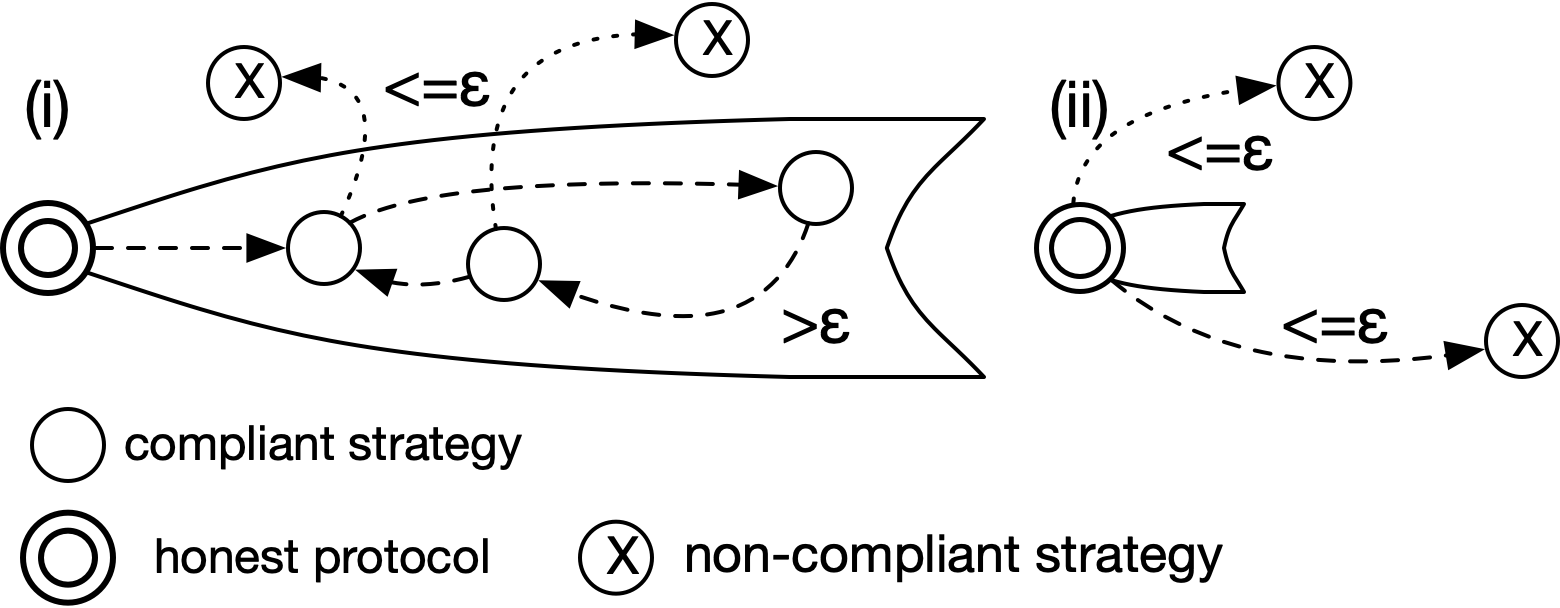
\includegraphics[width=0.8\columnwidth]{figures/compliance/cone.png}
    \end{center}
    \caption{
        Illustration of a compliant protocol that does not exhibit an
        equilibrium (i), vs a protocol which is an approximate Nash equilibrium
        (ii).
    }
    \label{fig:cone}
\end{figure}

First, Section~\ref{sec:model} describes our model of \emph{compliant}
strategies and protocols. A strategy is compliant if a party that employs it
never violates a predicate $\infractionPredicate$, which captures well-defined
types of deviant behavior. Accordingly, a protocol is compliant if, assuming a
starting point where no party deviates, no party will eventually employ a
non-compliant strategy, assuming sequential unilateral defections.
Section~\ref{sec:blockchains} specifies compliance for blockchain protocols,
under an infraction predicate that captures abstaining and producing
conflicting blocks, and two types of utility, absolute rewards and profit.
Following, we explore different reward schemes and families of protocols.
First, Section~\ref{sec:universal} shows that \emph{fair} rewards, \ie which
depend only on a party's mining or staking power, result in compliance \wrt
rewards alone (i.e., when costs are negligible), but non-compliance \wrt profit
(rewards minus costs). Next, we explore block-proportional rewards, \ie which
depend on the blocks adopted by an impartial observer of the system.
Section~\ref{subsec:bitcoin} shows that PoW systems are compliant \wrt rewards.
Section~\ref{subsec:single-leader-pos} shows that PoS systems, which enforce
that a single party participates at a time, are compliant, under a synchronous
network, but non-compliant under a lossy network.
Section~\ref{subsec:multi-leader-pos} shows that PoS systems, which allow
multiple parties to produce blocks for the same time slot, are not compliant.
Notably, our negative results show that a party can gain a
\emph{non-negligible} reward by being non-compliant. Finally, we evaluate
compliance under various externalities, \ie an exchange rate, which models
real-world prices, and external rewards, which come as a result of successful
attacks. We show that, historically, the market's response is not sufficient to
disincentivize attacks, so penalties should be necessary, for the level of
which we provide estimations based on the ledger's parameters and the market's
expected behavior.
